\subsubsection{State Charts}
In this section, state charts are employed in order to provide support to the reader in understanding how the internal states of some domain components change over time. In particular, the focus is on the Tournament and Battle entities.\\[0.7cm]

\textbf{Tournament State Chart}

   \begin{center}
    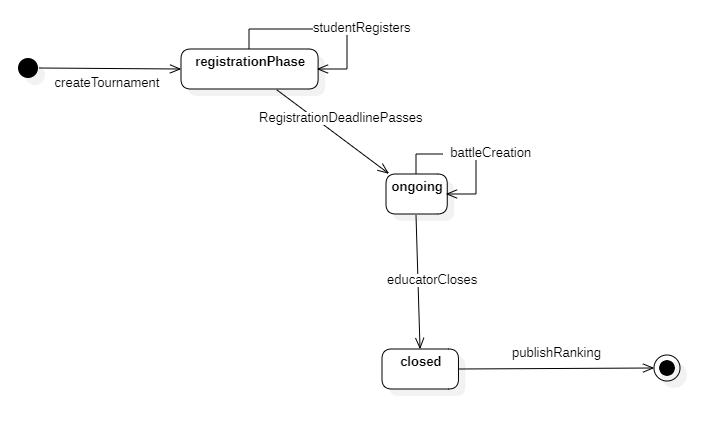
\includegraphics[width=1\textwidth]{2Overall_Description/res/StateChartTournament}
    \end{center}

After an educator creates a new tournament, all students with an account on \app are notified and can subscribe to it. This is the \textbf{registrationPhase} state. When the registration deadline passes, the tournament starts and students can no longer sign up. The state is now \textbf{ongoing} and this is the phase in which battles are created inside the tournament by educators. When the educator that created the tournament decides to close it, the tournament moves to the \textbf{closed} state. At this point, no more battle can be published in the tournament and the final ranking of fstudents is released.\\

\begin{minipage}{\linewidth}
\textbf{Battle State Chart}

\begin{center}
    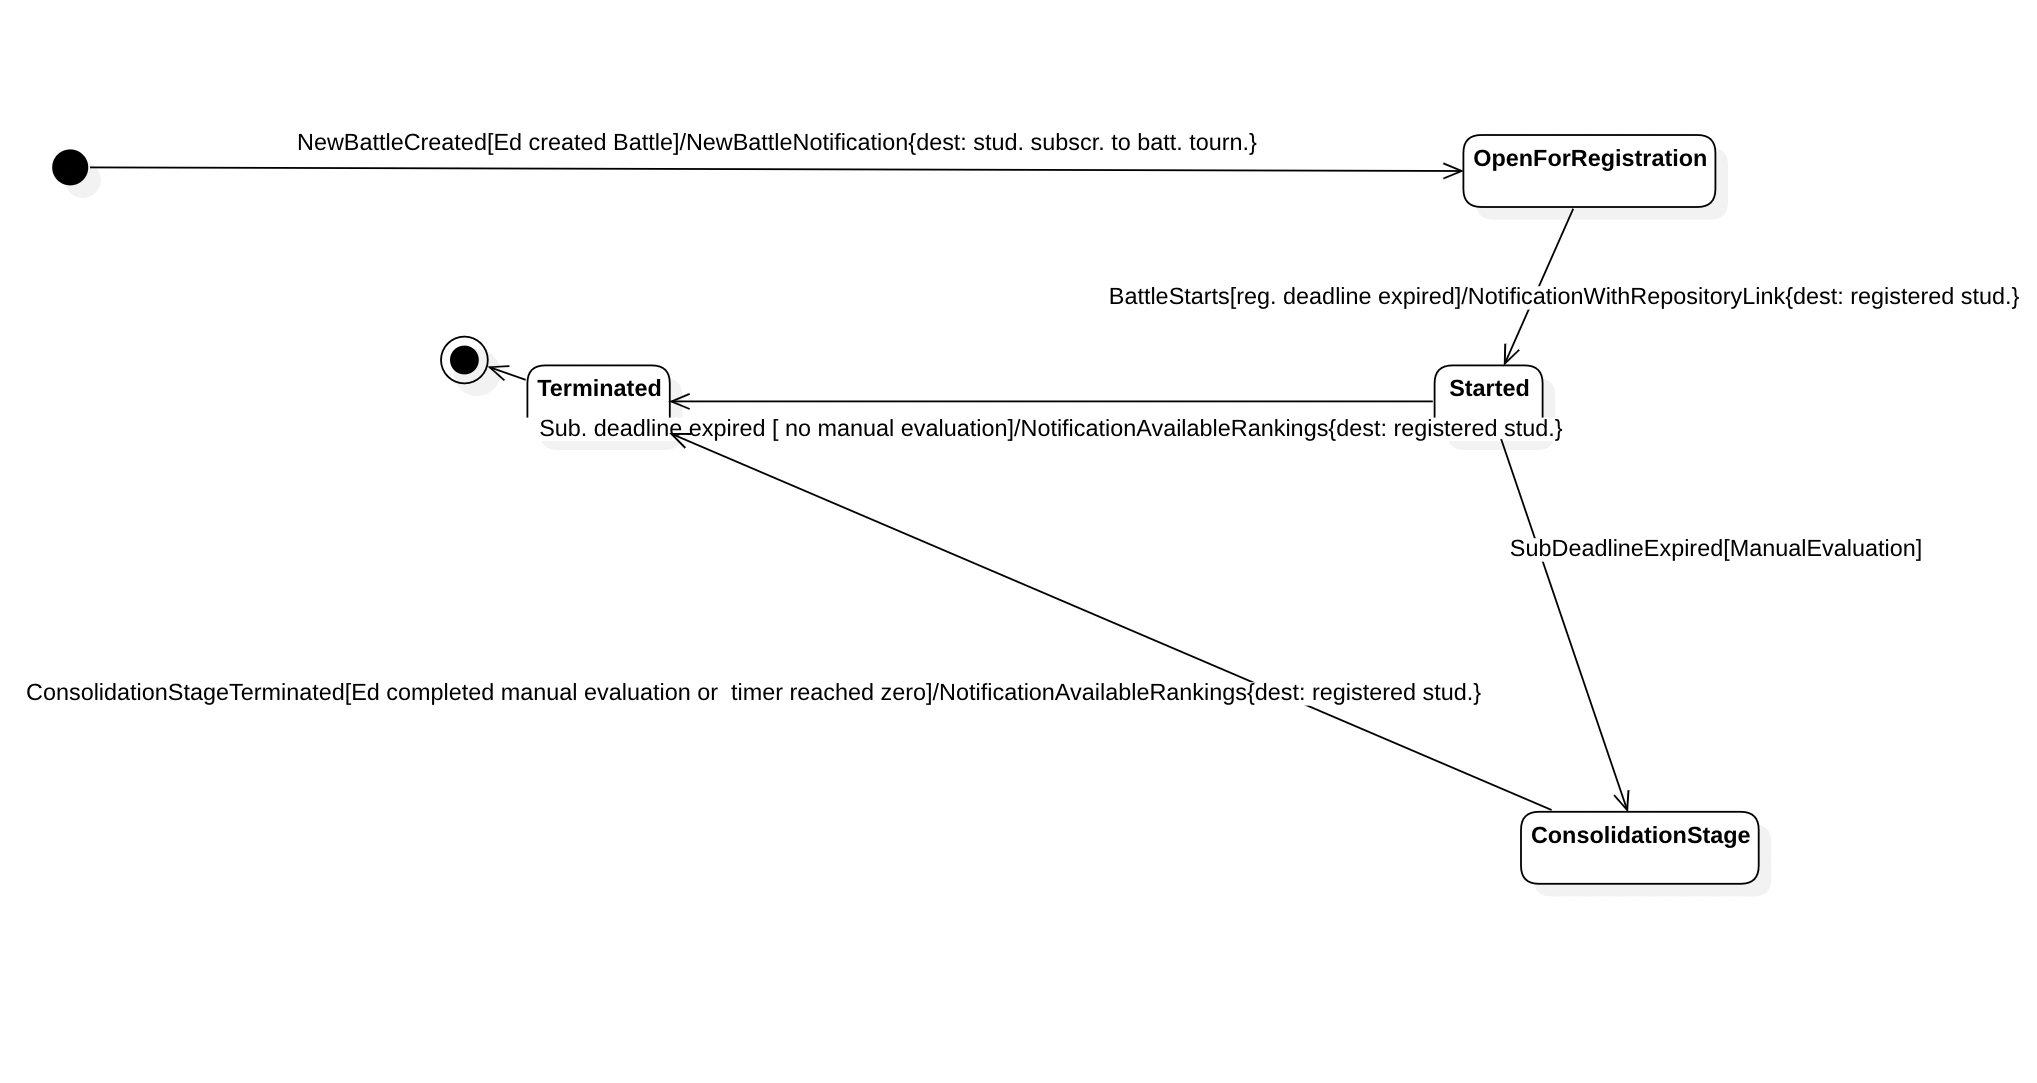
\includegraphics[width=1\textwidth]{2Overall_Description/res/stateChartBattle.png}
\end{center}
\end{minipage}

When a battle is created by an educator, it is in the \textbf{registrationPhase} state, during which students can join the battle. When the registration deadline passes, the battle moves on to the \textbf{ongoing} state. In this state, students can no longer sign up for the battle and the students who decided to participate are able to submit their code solutions through GitHub. When the submission deadline is met, there are two possible cases. If the educator who created the battle didn't request the consolidation stage for the battle, then the battle can simply terminate (\textbf{terminated} state) and the final ranking is published. On the other hand, if the professor who created the battle requested the consolidation stage, then the state shifts to \textbf{consolidationStage}. In this state, \app initiates a timer to set a time frame for the educator to manually evaluate the students' code solutions. When the timer goes off, if all teams of the battle received an evaluation from the educator, then the scores assigned during the consolidation stage are taken into account to compute the final ranking, otherwise \app will ignore the consolidation stage and publish the ranking based on the scores obtained in the \textbf{ongoing} state.
\clearpage


